\section{Verification purpose}

\textbf{Case ID:} \CaseID

This case verifies the limiting mechanism shared by steady Eulerian transport and zero-delay wildland ignition. The \texttt{transport\_impulse} variant disables surface spread and uses an areal source; \texttt{wildland\_no\_delay} uses a fire-power-based source and additionally checks accumulated population.

The paired design exposes failures in generation, transport, deposition, direct ignition, and time-of-arrival updates. Success requires both variants to recover wind-speed arrival behavior and the wildland variant to recover its one-metre-strip accumulation reference.

\section{Mathematical formulation and numerical implementation}
For constant wind speed $U=6.71$~m/s and zero ignition delay, an ember-deposited
cell becomes an active source immediately. Translation invariance then gives
\begin{equation}
 t_{\rm ref}(x)=\frac{x-x_0}{U},\qquad
 x_{\rm LE,ref}(t)=x_{\rm LE,0}+U(t-t_0),\qquad
 \overline{ROS}_{\rm ref}=U,
 \label{eq:transport}
\end{equation}
where $x_0$ is the first usable cell centre. The final arrival-time raster stores
the complete cell-crossing history used for the TOA profile metric. Leading-edge
history is evaluated independently from every dumped instantaneous level-set
field. At the physical centre row, the postprocessor linearly interpolates every
adjacent pair of cell-centred $\phi$ values that changes sign and retains the
rightmost $\phi=0$ crossing. Here $x_{\rm LE,0}$ is the first extracted crossing
at dump time $t_0$. Once the zero contour has left the physical domain, that dump
has no observable in-domain leading edge and is excluded from the trajectory fit
rather than being replaced by a stationary domain-edge value. Mean ROS is the
least-squares slope through all observable dump samples.

For immediate-ignition variant, a burning cell emits during its surface-fire residence time. Using
the FLIN and spread rate written by the same executed cell gives
\begin{equation}
 t_{\rm emission}=\frac{\Delta x}{VS},\qquad
 N_{\rm ref}=GR_{1m}\,\frac{FLIN}{1000}\,\frac{\Delta x}{VS}.
 \label{eq:accumulation}
\end{equation}
Here FLIN is in kW\,m$^{-1}$ and VS is converted from ft\,min$^{-1}$ to
m\,s$^{-1}$. The documented nominal FLIN and VS give 1497.2 particles
for this illustrative state~\cite{Qin2025}; the metric uses run-derived values
so it remains consistent with the active fuel calculation.
ELMFIRE forms pixel fire power from fireline intensity times cross-stream width
$\Delta y$. The configured coefficient $GR_{\rm ELM}=33.3/\Delta y$
pcs/s/MW therefore makes the raw pixel count represent a one-metre strip.
For the one-dimensional unit-width profile, each centre-row pixel count is
converted to the density of the represented one-metre strip,
\begin{equation}
n_i=\frac{N_i}{\Delta x(1\ {\rm m})}\quad[\mathrm{pcs\,m^{-2}}].
\label{eq:density}
\end{equation}
The two-cell numerical halo is excluded. The complete physical raster is still
inspected, and its all-row deposited total is retained as a conservation
diagnostic, but it is not mixed into the one-dimensional plotted observable.
For the PER-AREA variant, the configured source gives
$n_\infty=GR\Delta x\tau_{\rm ember}/(1~\mathrm{m})$. For the PER-MW
variant, Equation~\ref{eq:accumulation} divided by
$\Delta x(1~\mathrm{m})$ gives the run-derived density reference.

The discrete algorithm is: generate embers in every active source cell; distribute
them among downwind bins; accumulate them in landing cells; apply DIRECT ignition
with $P_{ign}=1$ and zero local/cell delay; update ember-ignition, level-set, and
TOA states together; then advance the level-set clock. The two variants differ
only where required by their source experiment.

\section{Derivation of expected behavior}
A deposition distribution with finite support changes which upstream cells
contribute near $x_0$, but not the propagation characteristic in
Equation~\ref{eq:transport}. Consequently TOA should be linear, and the leading
edge extracted from $\phi$ should oscillate by at most one cell around
$x_{\rm LE,0}+U(t-t_0)$. Its fitted slope should approach $U$. Every cell marked by the
ember-ignition raster must have finite nonnegative TOA.

In both variants, locations farther than the maximum travel distance receive
contributions from a complete set of upstream emitters. Conservation then produces
the configuration-consistent plateaus. The PER-AREA source uses
$GR=10$~pcs~m$^{-2}$~s$^{-1}$, $\Delta x=10$~m, and
$\tau_{\rm ember}=6$~s, giving 600~pcs~m$^{-2}$ under the represented-strip
normalization. The PER-MW reference is calculated from co-located final FLIN
and VS. The 155--195~m interval contains cells with complete upstream support.

\section{Verification metrics and acceptance criteria}
For valid centre-row cells, define $e_i=|t_i-t_{\rm ref,i}|/t_{\rm ref,i}$.
Each variant requires at least two cells, $\bar e\le0.10$, and
$\max e_i\le0.25$. Leading-edge error is the RMSE relative to
$x_{\rm LE,0}+U(t-t_0)$ divided by $U(t_{\rm last}-t_0)$ and must not exceed
0.10; $t_{\rm last}$ is the last dump with an in-domain $\phi=0$ crossing.
Every scheduled time must have exactly one matching $\phi$ raster. Fitted mean-ROS relative
error must not exceed 0.10. All ember-ignited physical cells must have finite, nonnegative TOA.
Each variant additionally requires
$|\widetilde n-n_{\rm ref}|/n_{\rm ref}\le0.10$, where
$\widetilde n$ is the median centre-row density from Equation~\ref{eq:density}
over the fully developed 155--195~m plateau. The corresponding analytical or
run-derived reference is calculated independently of the ember-flux values.
Domain-wide deposited totals are also recorded as diagnostics. Exactly two
manifest variants and one final raster of every required
kind are mandatory. The overall decision is the conjunction of completeness and
all component decisions; missing or stale products are non-passing.

\subsection{Justification of metric quantification}

The 10\% limits on mean TOA, leading-edge NRMSE, fitted ROS, and plateau
density are engineering verification bands for a first-order, cell-centred
transport/ignition calculation.  They are broad enough to accommodate
grid-crossing time quantization and the use of a localized run-derived FLIN/VS
reference, yet they remain small compared with the order-one signature of a
nonpropagating or solver-step-limited implementation.  The 25\% pointwise TOA
limit is intentionally looser than the mean limit because a single cell next
to the source or front can carry a disproportionately large relative timing
error; requiring at least two cells and the 10\% mean prevents that allowance
from masking a systematic bias.  The plateau median is used because the
expectation is spatially constant and the median is insensitive to one raster
edge cell.  Ignition-state consistency has zero physical tolerance: a cell
cannot be classified as ember ignited without a finite, nonnegative arrival
time.  Both variants and all components are conjunctive because transport,
ignition, and accumulation are separate claims of this combined test.

\subsection{Predeclared acceptance contract}

Table~\ref{tab:acceptance-contract} summarizes the metrics fixed before
inspection of the calculated results. Numerical values and component statuses
are reported separately in Section~7.

\begin{table}[H]
\centering
\footnotesize
\caption{Predeclared verification metrics and acceptance criteria.}
\label{tab:acceptance-contract}
\begin{tabular}{@{}p{0.23\linewidth}p{0.47\linewidth}p{0.21\linewidth}@{}}
\toprule
Metric & Output, region, and aggregation & Acceptance criterion\\
\midrule
Output completeness & Two manifest variants with one final TOA, ignition-state, and accumulated-firebrand product of each required kind, plus one $\phi$ raster for every scheduled dump time. & 2 of 2 variants complete; no missing $\phi$ dumps \\
TOA profile error & Mean and maximum of \(|t_i-t_{ref,i}|/t_{ref,i}\) on valid centre-row physical cells. & Mean \(\le0.10\); maximum \(\le0.25\) \\
Leading-edge error & RMSE of the rightmost interpolated $\phi=0$ crossing relative to \(x_{LE,0}+U(t-t_0)\), normalized by the observable reference displacement. & \(\mathrm{NRMSE}\le0.10\) \\
Mean-ROS error & Relative error of fitted leading-edge ROS against \(U=\SI{6.71}{m.s^{-1}}\). & \(\le0.10\) \\
Ignition-state consistency & Every ember-ignited physical cell has a finite, nonnegative TOA. & No inconsistent cells \\
Accumulation plateau error & Relative error of median one-metre-strip density over 155--\SI{195}{m} against the independent reference. & \(\le0.10\) for both variants \\
Overall decision & Conjunction of completeness and every component for both variants. & PASS only if all pass \\
\bottomrule
\end{tabular}
\end{table}

\section{Simulation configuration and predicted outcome}

Figure~\ref{fig:input-configuration} records the prepared spatial inputs for \texttt{transport\_impulse}.
The postprocessor reads these panels from the variant-local GeoTIFF files, removes the
two-cell numerical buffer, and retains map coordinates in metres.  The left panel shows
the most informative fuel or structure layout available for the case; the right panel
shows the cells selected by the non-positive initial level-set field, making a localized
ignition or firebrand-emission source explicit.

\begin{figure}[H]
\centering

\includegraphics[width=0.98\textwidth,height=0.42\textheight,keepaspectratio]{../figures/input_configuration.pdf}
\caption{Whole-domain prepared input configuration for the representative variant.  The
physical domain is shown without the numerical halo; coordinates, configured wind values,
fuel or structure layout, and initial ignition/source geometry are identified in the panels.}
\label{fig:input-configuration}
\end{figure}

\begin{table}[!htbp]\centering\small
\begin{tabular}{p{0.24\textwidth}p{0.27\textwidth}p{0.12\textwidth}p{0.265\textwidth}}
\toprule Parameter & Configured value & Units & Verification role\\ \midrule
Domain & $500\times100$ & m & common physical extent\\
Grid and halo & $10$; two cells/side & m & prescribed resolution; excluded halo\\
Time step & $0.5\Delta x/U=0.745$ & s & wind CFL 0.5\\
Wind & $6.71$, from $270^\circ$ & m/s & constant transport velocity\\
Fuel/terrain & FBFM 102; flat & -- & uniform wildland control\\
Transport variant & PER-AREA; surface off; 100 s & -- & isolates transport-impulse variant transport\\
Wildland variant & PER-MW; surface on; 100 s & -- & immediate-ignition variant residence source\\
Transport/ignition & EMPIRICAL;\newline EULERIAN; DIRECT & -- & current spotting path\\
Ignition response & $P_{ign}=1$; delays zero & -- & immediate limiting regime\\
Crosswind/consumption & disabled/disabled & -- & one-dimensional conservation\\
\bottomrule
\end{tabular}
\caption{Configuration shared by and distinguishing the two combined variants.}
\end{table}
\FloatBarrier

Before inspecting output, both TOA curves should overlay $(x-x_0)/U$. Both
dumped-$\phi$ leading-edge histories should follow
$x_{\rm LE,0}+U(t-t_0)$ with grid-scale steps, and their
mean ROS should be near 6.71~m/s. The two density bar profiles should rise near
the inlet and approach their horizontal references: 600~pcs~m$^{-2}$ for the
PER-AREA transport variant and the FLIN/VS-derived value for the wildland variant.
\section{Actual simulation results}

Figure~\ref{fig:domain-result} shows the representative accumulated firebrand density from \texttt{transport\_impulse}.
It is read from the actual ELMFIRE output named in the panel, masks nodata, and excludes
the two-cell numerical buffer.  Firebrand counts are normalized by the cell length and the represented 1-m cross-stream strip, giving units of pcs m$^{-2}$.

\begin{figure}[H]
\centering

\includegraphics[width=0.96\textwidth,height=0.50\textheight,keepaspectratio]{../figures/domain_result.pdf}
\caption{Whole-domain accumulated firebrand density from the representative completed ELMFIRE run.  This
domain-scale result supplements, rather than replaces, the higher-level verification
profiles, convergence plots, ensemble statistics, and calculated acceptance metrics below.}
\label{fig:domain-result}
\end{figure}


The runner regenerated both input stacks and postprocessed only the current
ELMFIRE products recorded in \path{variants/manifest.json}.
Figure~\ref{fig:steady-reference} presents the four physical observables
used in the steady-transport reference experiment: accumulated density, arrival
time, leading-edge position, and instantaneous leading-edge rate of spread.

\begin{figure}[H]
\centering
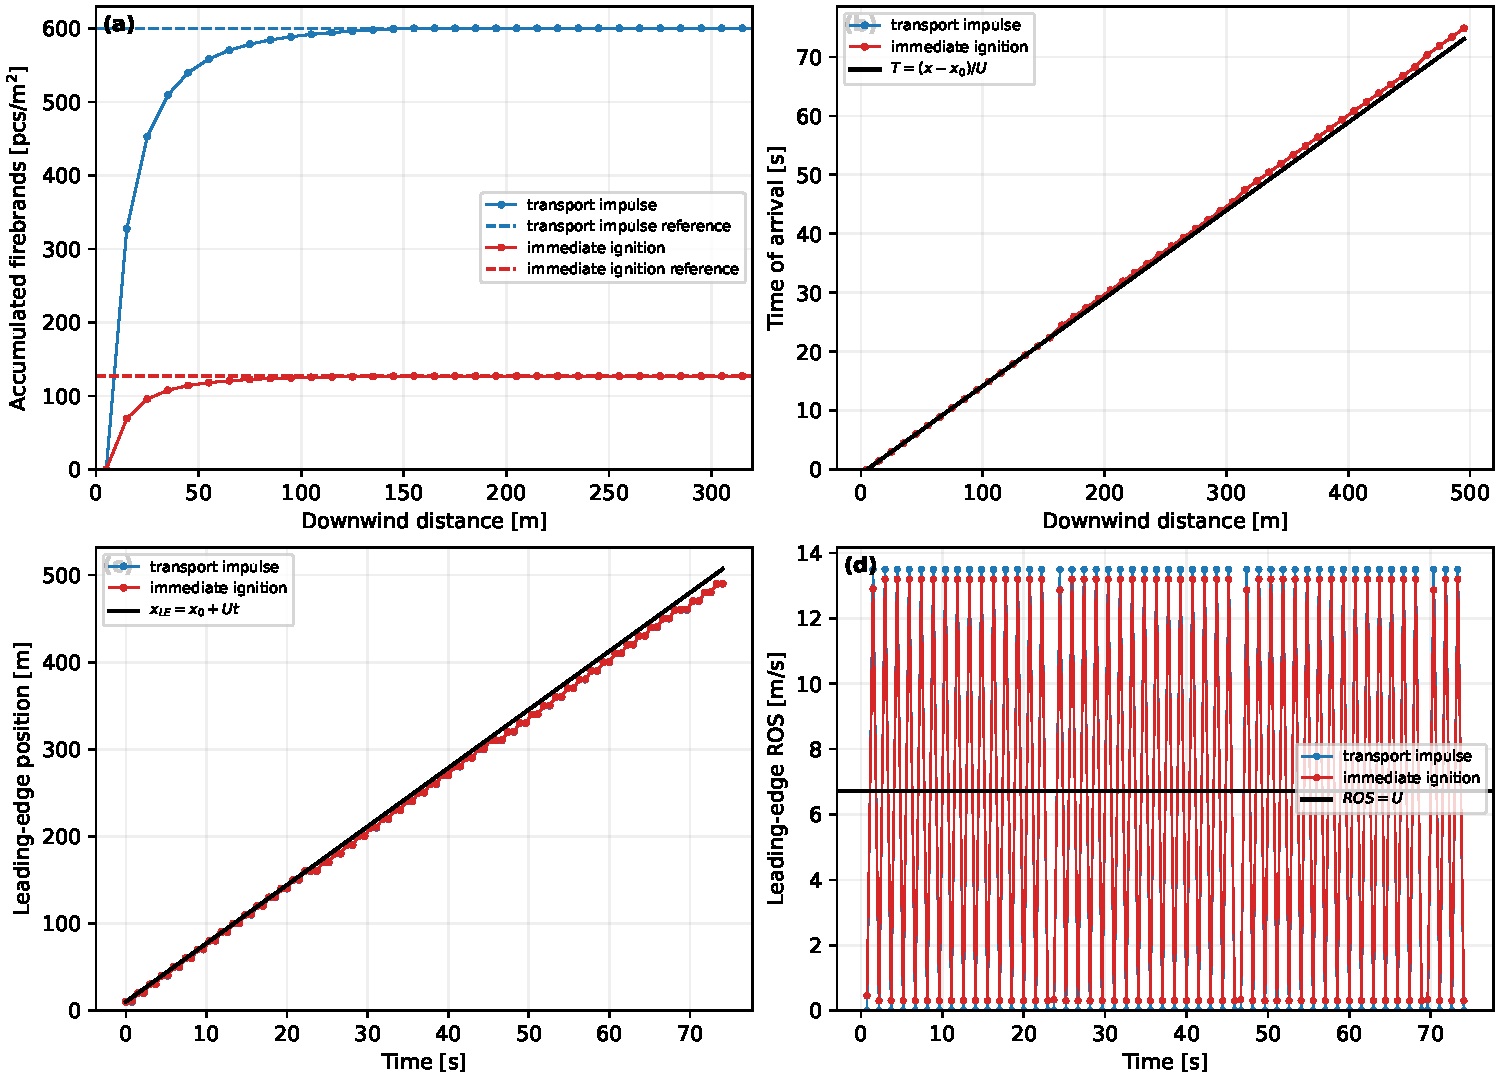
\includegraphics[width=0.98\textwidth,height=0.68\textheight,keepaspectratio]{../figures/steady_transport_reference.pdf}
\caption{Steady-transport and immediate-ignition observables from actual
ELMFIRE outputs. Solid colored curves identify the two controlled variants;
black or color-matched reference curves show the derived analytical behavior.}
\label{fig:steady-reference}
\end{figure}

\FloatBarrier

\section{Calculated metrics and verification decision}
\begin{table}[!htbp]\centering\small
\begin{tabular}{llll}\toprule
Metric & Limit & Calculated & Status\\ \midrule
Output completeness & 2 variants & \Metric{evaluatedvariants}/\Metric{requiredvariants} & \Metric{outputcompletenesspassed}\\
Transport $\phi$ history & all scheduled dumps & \Metric{transportphidumpcount}/\Metric{transportscheduledphidumpcount} dumps; \Metric{transportphiobservablefrontcount} contours & \Metric{transportphidumpcompletenesspassed}\\
Transport TOA mean error & $\le0.10$ & \Metric{transporttoameanrelativeerror} & \Metric{transporttoapassed}\\
Transport leading-edge NRMSE & $\le0.10$ & \Metric{transportleadingedgenormalizedrmse} & \Metric{transportleadingedgepassed}\\
Transport mean-ROS error & $\le0.10$ & \Metric{transportmeanrosrelativeerror} & \Metric{transportmeanrospassed}\\
Wildland $\phi$ history & all scheduled dumps & \Metric{wildlandphidumpcount}/\Metric{wildlandscheduledphidumpcount} dumps; \Metric{wildlandphiobservablefrontcount} contours & \Metric{wildlandphidumpcompletenesspassed}\\
Wildland TOA mean error & $\le0.10$ & \Metric{wildlandtoameanrelativeerror} & \Metric{wildlandtoapassed}\\
Wildland leading-edge NRMSE & $\le0.10$ & \Metric{wildlandleadingedgenormalizedrmse} & \Metric{wildlandleadingedgepassed}\\
Wildland mean-ROS error & $\le0.10$ & \Metric{wildlandmeanrosrelativeerror} & \Metric{wildlandmeanrospassed}\\
Transport accumulation error & $\le0.10$ & \Metric{transportaccumulationrelativeerror} & \Metric{transportaccumulationpassed}\\
Wildland accumulation error & $\le0.10$ & \Metric{wildlandaccumulationrelativeerror} & \Metric{wildlandaccumulationpassed}\\
Transport deposited total & diagnostic & \Metric{transporttotalaccumulatedfirebrandsdomainpcs} pcs & --\\
Wildland deposited total & diagnostic & \Metric{wildlandtotalaccumulatedfirebrandsdomainpcs} pcs & --\\
Overall decision & all components pass & \Metric{verificationpassed} & \textbf{\Metric{status}}\\
\bottomrule\end{tabular}
\caption{Metrics read directly from \texttt{outputs/metrics.json}.}
\end{table}
\FloatBarrier

\section{Technical interpretation}
The combined decision distinguishes a transport defect from a source-duration or
normalization defect. Agreement in transport-impulse variant but not immediate-ignition variant implicates the
residence-time PER-MW path; disagreement in both implicates shared transport,
direct ignition, or TOA state handling. A full-area total of \Metric{wildlandtotalaccumulatedfirebrandsdomainpcs} particles was deposited across \Metric{wildlandactivedepositionrows} active rows. A plateau-only failure cannot be hidden
by a plausible TOA curve, and an average ROS cannot hide local TOA or product
inconsistency. The numerical values in the table and figure provide the executed
source revision's decision rather than a qualitative visual judgment.

\section{Scope and limitations}
This is deterministic code verification of steady one-dimensional Eulerian
transport and immediate ignition. It does not validate the empirical spotting
PDF against experiments, time-varying wind, crosswind transport, stochastic
ignition, delayed ignition, Lagrangian tracking, or consumption. Surface spread
is present in the immediate-ignition variant source calculation but the wind-speed leading edge is
expected to dominate. Run \texttt{./run\_case.sh} from any working directory to
regenerate both variants and the standalone report.

\begin{thebibliography}{9}
\bibitem{Qin2025}
Y. Qin, \emph{A Physics-Based Eulerian Framework for Modeling Firebrand
Showering in Regional-Scale Wildland and Wildland--Urban Interface Fire
Simulations}, Ph.D. dissertation, University of Maryland, College Park, 2025.
\end{thebibliography}
